\documentclass[a4paper, 12pt, notitlepage]{article}
\usepackage[utf8x]{inputenc}
\usepackage{titling}
\usepackage{blindtext}
\usepackage[nodayofweek]{datetime}
\usepackage{etoolbox}
\patchcmd{\formatdate}{,}{}{}{}
\date{}
\usepackage{multicol}
\usepackage[a4paper,left=48px,right=48px,top=50px,bottom=50px,
includefoot,heightrounded]{geometry}

\usepackage{titlesec}
\titleformat{\section}[block]{\Large\bfseries}{\thesection}{4mm}{}
\titleformat{\subsection}[block]{\large\bfseries}{\thesubsection}{2mm}{}
\titleformat{\subsubsection}[block]{\large\bfseries}{\thesubsubsection}{2mm}{}

\usepackage[shortlabels]{enumitem}

\usepackage{graphicx}
\usepackage{xcolor}
\graphicspath{ {./images/} }
\usepackage{caption}
\usepackage{subcaption}
\usepackage{amssymb}
\usepackage{amsmath}
\usepackage{hyperref}
\hypersetup{colorlinks=true, linkcolor=blue, citecolor=blue}
\usepackage{float}

\setlength{\columnsep}{40px}


\title{\Huge\textbf{Cooperative Object Transportation \\through an Unstructured Environment}}
\author{TORIELLI Davide \quad FUSARO Fabio \\\\
	\small EMARO - European Master on Advanced Robotics\\
	\small DIBRIS - Dip. Informatica, Bioingegneria, Robotica, Ing. Dei Sistemi\\
	\small Università Degli Studi Di Genova, \today}

\begin{document}

	\maketitle
	
	\begin{multicols}{2}
		\section*{Abstract}
		\textit{\hspace{7px}Cooperative manipulation and transportation 
		by means of multi-robot systems is a subject that has
		received an increased interest in the last few years. This work is focused on cooperation of two mobile robots (KUKA YouBot) in a difficult enviroment, each one with a 5-DOF arm on it, carrying a common load with their end-effectors. In particular we focused on the obstacle avoidance task.}
	
		\section{Introduction}
		\hspace{7px}The cooperation of multi-robot systems is a hot topic, important for many applications. There are situations in which a load is too big or too heavy to be carried by a single agent; so a collaboration among multiple agents for a safe and/or a physically possible transportation is necessary.\\
		In this work we focused on two mobile robots with arms, but the theory which we based on is applicable in many others fields (for example, submarine vehicles coordination \cite{subvec}).\\
		\hspace*{7px}The first step is to control the single robot. As seen in other works \cite{tpik}, this is done through a task priority inverse kinematic (TPIK) approach. This strategy permits the robot to accomplish various tasks in order of priority and it allows also to not consider one (or more) of them that are not important in a particular moment (for example, it is not necessary to avoid an obstacle if this is far away). \\
		Then this approach is extended to include the cooperation between the two robots, as in \cite{coopcasa} \cite{wander}.\ 
		The chosen approach is not a leader-follower one; here the agents help each other after understanding which one is in a more difficult situation (for example, a near obstacle). 
		Starting from here, we added a new task: the obstacle avoidance.\\
		The work was done in EMAROLAB of University of Genova, with two KUKA youBot running in a Motion Capture (MoCap) enviroment.\\
		\hspace*{7px}The paper is structured as follows. \\Section \ref{sec:scope} describes the aim of the project. Section \ref{sec:theory} recalls the theory of the used task priority framework. Section \ref{sec:oat} explains the development of the obstacle avoidance task and section \ref{sec:res} presents the  achieved experimental results. Finally, conclusions in section \ref{sec:conc} are given.
		
		\section{Scope of work}\label{sec:scope}
		\hspace{7px}We will now briefly explain the problem we have faced. As can be seen in Fig.\ \ref{fig:youBots} the two robots are approaching an obstacle. Obviously the aim is to avoid it with both robots.  
		This new task is added together with the other ones, like strictly keeping the load or avoiding singular positions, in the TPIK list.
		
		\begin{figure}[H]
			\centering
			\includegraphics[width=\linewidth]{youBots}
			\captionof{figure}{\small \textit{The youBots approaching the obstacle} }
			\label{fig:youBots}
		\end{figure}
		
		\hspace{-9px}As said previously, the robot used is the KUKA youBot that is a mobile robot composed by two parts: a mobile platform and an arm. The platform is an omnidirectional base with four mecanum wheels; the arm is a five degrees of freedoms manipulator with two-finger gripper \cite{kuka}.
		
		\section{Theory behind the work} \label{sec:theory}
		\hspace{7px} Here we summarize the theory explained deeper in \cite{coopcasa} and \cite{wander}.
		\subsection{Control Architecture}
		\hspace{7px} The control architecture for the single robot is represented in Fig.\ \ref{fig:controlArch}.
		There are three main blocks:
		\begin{enumerate}[leftmargin=*]
			\setlist{length\itemsep{0px}}
			\item The Mission Manager is the supervisor of the current \textit{mission} (i.e.\ sequence of actions $\mathcal{A}_j$) and generates the actions to be executed by the Kinematic Control Layer.
			\item The Kinematic Control Layer (KCL) is in charge of reactively accomplishing the \textit{control objectives} generating the desired system velocity vector.
			\item The Dynamic Control Layer (DCL) generates appropriate forces or torques to track the desired system velocity vector. 
		\end{enumerate}
		
		This work focuses on the KCL where the task priority approach is implemented. 
		
		\vspace{-10px}
		\begin{figure}[H]
			\centering
			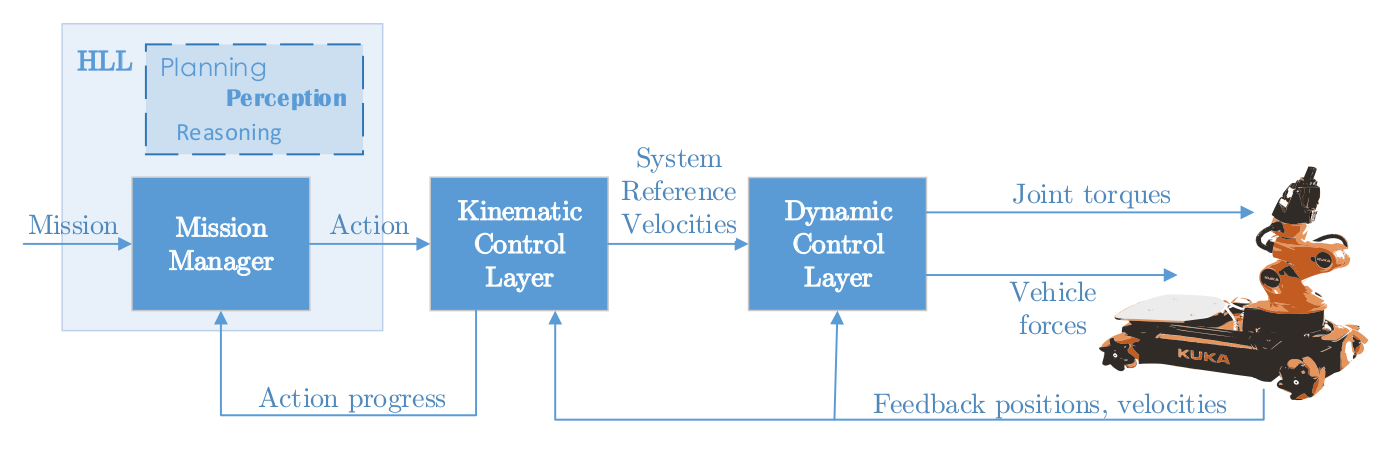
\includegraphics[scale=0.17]{controlArch}
			\captionof{figure}{\small \textit{The overall control architecture} }
			\label{fig:controlArch}
		\end{figure}
		
		\subsection{Single Agent}\label{subsec:sinag}
		\hspace{7px} In the following paragraphs, the robot configuration vector is referred to as $\boldsymbol{c} \triangleq [\boldsymbol{q} \quad \boldsymbol{\eta}]^T \:\in \,\mathbb{R}^n$ where $\boldsymbol{q} \in \,\mathbb{R}^l$ is the arm joint position vector and  $\boldsymbol{\eta} \, \in \,\mathbb{R}^6$ is the vehicle position and orientation vector. The robot velocity vector is named $\boldsymbol{\dot{y}} \triangleq [\boldsymbol{\dot{q}} \quad \boldsymbol{v}]^T \:\in \,\mathbb{R}^n$, and represents the controls to actuate the robot, e.g., joint velocities and vehicle linear and angular velocities. For the youBot mobile manipulators used in the experiments, both $\boldsymbol{\eta} \in \,\mathbb{R}^3$ and $\boldsymbol{v} \in \,\mathbb{R}^3$ consist only in the horizontal position and velocity, plus the yaw angle and its derivative.
		\subsubsection{Control Objective}
		\hspace{7px} Considering a scalar variable  $x_o(\textbf{c})$ related to a control objective \textit{o}, then:
		\begin{itemize}[leftmargin=*]
	
			\setlist{length\itemsep{0px}}
			\item The requirement, for t → $\infty$, that $x_o (\boldsymbol{c}) = x_{o,0}$ is called
			a scalar \textit{equality} control objective.
			\item The requirement, for t → $\infty$, that $x_o(\boldsymbol{c}) < x_{o,max}$ or
			$x_o(\boldsymbol{c}) > x_{o,min}$ is called a scalar \textit{inequality} control objective.
		\end{itemize}
		where $x_{o,0}$ is a given reference value and $x_{o,min}$ and $x_{o,max}$ are lower and upper thresholds among which the variable must stay.
		These requirements model the objectives that the system should satisfy, for example avoiding obstacle, respecting joint limits, reaching desired position.
		
		
		\subsubsection{Control Tasks} \label{subsubsec:contrTask}
		\hspace{7px} Remembering that the time behaviour of each scalar variable $x_o$ is related
		to the system velocity vector through a Jacobian relationship
		$\dot{x}_o = \boldsymbol{J}_o(\boldsymbol{c})\boldsymbol{\dot{y}}$, (where $\boldsymbol{J}_o(\boldsymbol{c}) ∈ \mathbb{R}^{1×n}$ is the Jacobian matrix
		of the task), the feedback reference rate $\dot{\bar{x}}_o$ is defined as	
		\begin{equation}
			\dot{\bar{x}}_o(x_o)\triangleq\gamma(x_o^* - x_o)  \quad with \:\gamma>0
		\end{equation}
		where $\gamma$ is a positive gain proportional to the desired convergence rate for the considered variable, and $x_o^*$ is a point inside the state region where \textit{o} is satisfied.\\The \textit{reactive control task} $\tau_0$ associated with the objective \textit{o} is defined as the need of minimizing the difference between the actual task velocity $\dot{x}_o$ and the feedback reference rate $\dot{\bar{x}}_o$. \\
		\hspace*{7px}There are cases where a control task is defined directly in	a certain task velocity space, without having an associated control objective. In such cases, there is
		no explicit control objective specified to the system and so we talk about \textit{non-reactive control task}.
		
		\subsubsection{Control Actions}
		\hspace{7px} From the robot control standpoint, an action $\mathcal{A}$ can be defined as a prioritized list of m control objectives $o_1,...,o_m$ each one with associated control task $\tau_1,...,\tau_m$. These tasks have to be managed \textit{concurrently} which means that we must satisfy the most prioritized objectives first and then, if possible, the others.

		
		\subsubsection{Activation Functions} \label{subsubsec:activFunc}
		\hspace{7px} Control objectives and their associated reactive control task are relevant depending on the current value of the system configuration vector \textbf{c}.
		For example, it is useless to over-constrain the system adding a task that avoid an obstacle that is far away. So, an \textit{activation function} is used 
		\begin{equation}\label{eq:act}
			a_o^i (x_o) \in [0,1]
		\end{equation}
		to \textit{activate / deactivate} the task. This is a continuous sigmoid function of the scalar objective variable $x_o$, whose value is zero when we are in the validity region of the associated control objective \textit{o}.\\
		For non-reactive control tasks, the variable $x(\boldsymbol{c})$ is not defined and the \eqref{eq:act} is simply $a_o^i (x_o) \equiv 1$.\\
		\hspace*{7px}When we talk about different actions $\mathcal{A}_j$, the \eqref{eq:act} is modified to become
		\begin{equation}
			a_o(x_o, \boldsymbol{p}) = a_o^i (x_o) a_o^p(\boldsymbol{p})
		\end{equation}
		where $a_o^p(\boldsymbol{p})\in [0,1]$ is an additional continuous sigmoid function of a vector of parameters p external to the control
		task itself, which can be can be conveniently parametrized to obtain the desired activation/deactivation smooth transition between different actions.
		
		
		\subsubsection{Task Priority Inverse\\ Kinematics}
		\hspace{7px} For an action  $\mathcal{A}$ we define:
		\begin{itemize}[leftmargin=*]
			\setlist{length\itemsep{0px}}
			\item $  \dot{\bar{\boldsymbol{x}}}_k \triangleq [   \dot{\bar{x}}_{1,k},...,\dot{\bar{x}}_{m,k}   ]^T $ is the stacked vector of all the reference rates, where the first index indicates control task $\tau_1,...,\tau_m$ placed at the priority level \textit{k}.
			\item $\boldsymbol{J}_k$ is the Jacobian relationship expressing the current rate
			of change of the \textit{k}-th task vector $[\dot{x}_{1,k},...,\dot{x}_{m,k}]^T$  with
			respect to the system velocity vector $\dot{\boldsymbol{y}}$.
			\item $\boldsymbol{A}_k \triangleq diag(a_{1,k},...,a_{m,k})$ is the diagonal matrix of all the activation functions in the form of \eqref{eq:act}.
		\end{itemize}
		
		Now, the control problem is to find the system velocity reference vector $\dot{\bar{\boldsymbol{y}}}$ that satisfies \textit{at best} the requirements. As in \cite{coopcasa}, this is expressed by the following minimization problems:
		\begin{equation}
			S_k \triangleq \Big\{ arg\:R\mbox{-} \; \min\limits_{\dot{\bar{\boldsymbol{y}}} \in S_{k-1}} \big\| \boldsymbol{A}_k (\dot{\bar{\boldsymbol{x}}}_k - \boldsymbol{J}_k \dot{\bar{\boldsymbol{y}}}) \big\|^2 \Big\}
		\end{equation}
		where $S_{k-1}$ is the manifold of solutions of all the previous
		tasks in the hierarchy, which means that $S_0 \triangleq \mathbb{R}$.
		
		\subsubsection{Vehicle-Arm Coordination}\label{subsubsec:vehArmcoord}
		\hspace{7px} If the whole body Jacobian were employed to control the end-effectors, disturbances of the mobile platform would propagate immediately through the coupled kinematics to the end effectors.
		To cope with this problem, the idea of \cite{coopcasa} is to have two TPIK procedures running in parallel as depicted in Fig.\ \ref{fig:veharmcoord}.
		
		\hspace{-30px}
		\begin{figure}[H]
			\centering
			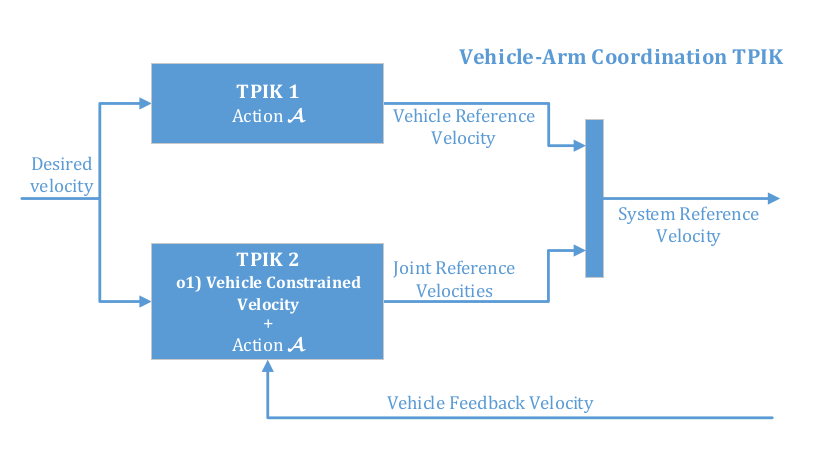
\includegraphics[scale=0.3]{veharmcoord}
			\captionof{figure}{\small \textit{Vehicle-Arm coordination scheme for action $\mathcal{A}$} }
			\label{fig:veharmcoord}
		\end{figure}
			
		\begin{enumerate}[leftmargin=*]
			\setlist{length\itemsep{0px}}
			\item \textbf{TPIK 1} considers the vehicle together with the manipulator. Of the whole result $\dot{\bar{\boldsymbol{y}}}$,
			only the vehicle reference velocity is used, while the
			manipulator part is discarded.
			\item \textbf{TPIK 2} considers the vehicle
			as a \textit{non-controllable} entity. A \textit{non-reactive} control task is added with the highest priority. Its role is to constrain the desired vehicle velocities equal to the \textit{current measured} ones. The outputs of this procedure are the \textit{optimal} joint velocities in correspondence of the \textit{measured} vehicle velocity.
		\end{enumerate}
		\vspace{-2px}
		Thanks to the TPIK 2 optimization, the arm joint velocities are always the optimal ones based on the current vehicle velocity, independently of any vehicle inaccuracy in tracking the desired one generated by TPIK 1.
		Also, this method copes with multi-rate control requirements of the two different subsystems.		
		
		\subsection{Cooperative Agents} \label{subsec:coopagents}
		\hspace{7px} We now focus on the case of multiple cooperative mobile manipulators; for simplicity we will consider two robots but the approach can be applied to multiple agents.
		
		\subsubsection{Introduction}
		\hspace{7px} Assuming a firm object grasping by part of two agents \textit{a},\textit{b}, the tool control points $\langle t_a \rangle$, $\langle t_b \rangle$ are assigned by the agents to coincide with the shared object fixed frame $\langle o \rangle$, that is $\langle t_a \rangle \equiv \langle t_b \rangle \equiv \langle o \rangle \triangleq \langle t \rangle$, as exemplified in Fig.\ \ref{fig:coopframes}.
		 
		\begin{figure}[H]
			\centering
			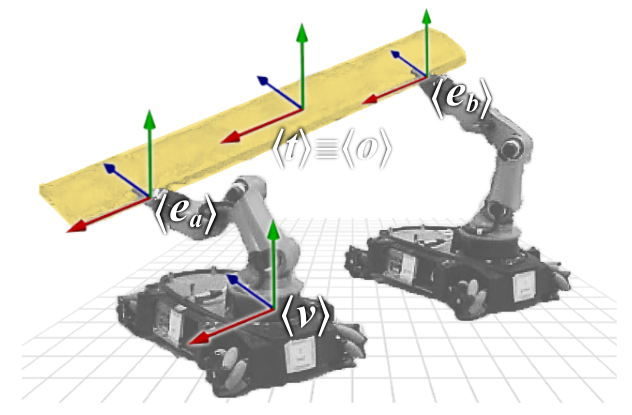
\includegraphics[scale=0.37]{coopFrames}
			\captionof{figure}{\small \textit{Frames involved in the cooperative mobile manipulation} }
			\label{fig:coopframes}
		\end{figure}
		
		\begin{figure*}[b]
			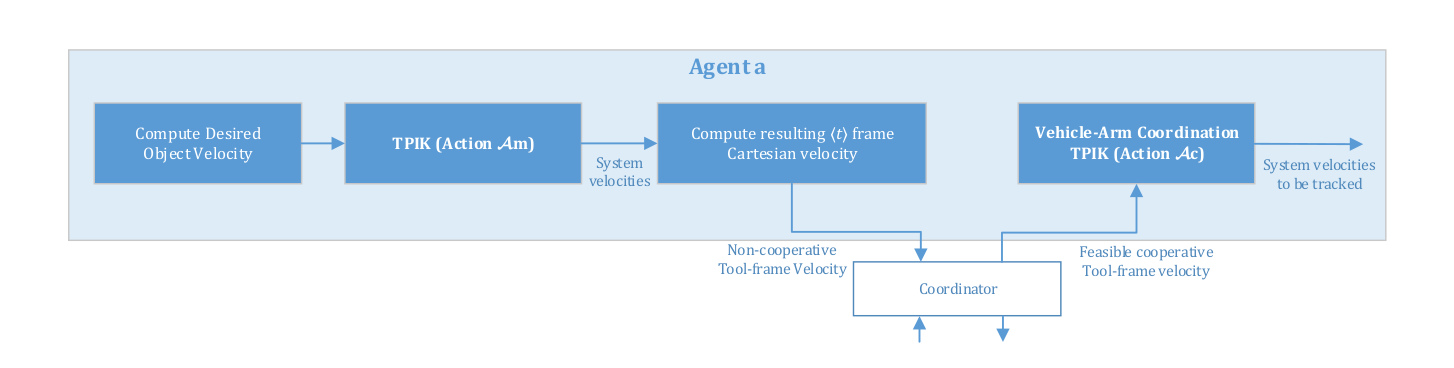
\includegraphics[width=\linewidth]{coop}
			\captionof{figure}{\small \textit{Block diagram of the cooperation, as seen from agent} a}
			\label{fig:coop}
		\end{figure*}
		
		In these conditions, the following differential constraints are imposed as consequence of the geometric ones:
		\begin{equation}\label{eq:coopintro}
		\dot{\boldsymbol{x}}_t = \boldsymbol{J}_{t,a} \dot{\boldsymbol{y}}_a = \boldsymbol{J}_{t,b} \dot{\boldsymbol{y}}_b,
		\end{equation}
		with $\dot{\boldsymbol{x}}_t$ the object velocity with components on $\langle t \rangle$ and $\boldsymbol{J}_{t,a}$, $\boldsymbol{J}_{t,b}$ the system Jacobians with respect to $\langle t \rangle$.\\Let us rewrite the second equation in \eqref{eq:coopintro} as
		\begin{equation}\label{eq:coopintro2}
		\begin{gathered}
		\begin{bmatrix}
		\boldsymbol{J}_{t,a} & -\boldsymbol{J}_{t,b}
		\end{bmatrix}
		\begin{bmatrix}
		\dot{\boldsymbol{y}}_a \\ \dot{\boldsymbol{y}}_b
		\end{bmatrix}
		\triangleq \boldsymbol{G}\dot{\boldsymbol{y}}_{ab}=0 \Longleftrightarrow \\ \dot{\boldsymbol{y}}_{ab} \in ker(\boldsymbol{G}),
		\end{gathered}
		\end{equation}
		which represents the subspace where $\boldsymbol{\dot{y}}_{ab}$ is constrained to lay as a consequence of the firm grasp assumption. \\
		Before proceeding with the coordination policy, let us consider the subspace of admissible Cartesian velocities of both systems which derived from \eqref{eq:coopintro2} by eliminating the internal motion components within each subsystems
		\begin{equation}
		(\boldsymbol{J}_{t,a} \boldsymbol{J}^\#_{t,a} - \boldsymbol{J}_{t,b} \boldsymbol{J}^\#_{t,b}) 
		\dot{\boldsymbol{x}}_t \triangleq \boldsymbol{C} \dot{\boldsymbol{x}}_t = \boldsymbol{0}
		\end{equation}
		thus implying $\dot{\boldsymbol{x}}_t \in ker(\boldsymbol{C}) = Span(\boldsymbol{I} - \boldsymbol{C}^\#\boldsymbol{C})$, where the kernel of the matrix $\boldsymbol{C}$ expresses the space of achievable object velocities at the current configuration. Therefore, if a desired object velocity $\dot{\tilde{\boldsymbol{x}}}_t$ lying in this subspace is commanded separately to both agents and the corresponding non-reactive end-effector velocity tracking task is located at the highest priority in both agents task priority lists, then the object kinematic constraint is satisfied at kinematic level.\\
		We now proceed with the description of the coordination policy.	
		
		\subsubsection{Coordination Policy}
		
		\hspace{7px} During each sampling interval, the following sequential steps are executed, as sketched in Fig.\ \ref{fig:coop} :
		
		\begin{enumerate}[leftmargin=*]
			\setlist{length\itemsep{0px}}
			
			\item Each agent runs the TPIK procedure detailed in subsection \ref{subsec:sinag} as if it were the only one acting on the object. The two TPIK procedures separately provide the vectors $\dot{\boldsymbol{y}}_a$, $\dot{\boldsymbol{y}}_b$.
			
			\item Each agent evaluates the Cartesian \textit{non-cooperative} tool-frame velocities
			\begin{equation}
				\dot{\boldsymbol{x}}_{t,i} = \boldsymbol{J}_{t,i} \dot{\boldsymbol{y}}_i , \quad i = a,b
			\end{equation}
			
			Moreover, each one evaluates the matrix $\boldsymbol{J}_{t,i} \boldsymbol{J}^\#_{t,i}$
			which is the representation of the admissible tool-frame velocity space.
			
			\item Both agents transfer their computed quantities to the Coordinator.
			
			\item The Coordinator performs the following steps:
			
			\begin{enumerate}[a), leftmargin=*]
				\setlist{length\itemsep{0px}}
				\item It evaluates the cooperative tool-frame velocity vector
				\begin{equation}\label{eq:weightsum}
					\begin{gathered}
					\dot{\hat{\boldsymbol{x}}}_t = \dfrac{1}{\mu_a + \mu_b} (\mu_a \dot{\boldsymbol{x}}_{t,a}  + \mu_b \dot{\boldsymbol{x}}_{t,b}),\\
					\mu_a , \mu_b > 0	
					\end{gathered}
				\end{equation}
				which corresponds to a weighted compromise between
				the two output velocities $\dot{\boldsymbol{x}}_{t,a} , \dot{\boldsymbol{x}}_{t,b}$.
				In the general case, i.e. $\dot{\boldsymbol{x}}_{t,a} \neq \dot{\boldsymbol{x}}_{t,b}$, the \eqref{eq:weightsum} might not lay in the space of feasible object velocities, therefore it must be projected on this subspace, as performed in the next two steps. 
				
				\item It evaluates the Cartesian constraint matrix
				\begin{equation}
					\boldsymbol{C} \triangleq \Big( \boldsymbol{J}_{t,a} \boldsymbol{J}^\#_{t,a} - \boldsymbol{J}_{t,b} \boldsymbol{J}^\#_{t,b} \Big)	
				\end{equation}
				
				\item It projects the evaluated cooperative velocity vector $\dot{\hat{\boldsymbol{x}}}_t$
				on the feasible velocity space $Span(\boldsymbol{I} − \boldsymbol{C}^\# \boldsymbol{C})$ for the constrained object, obtaining the so-called \textit{feasible cooperative} velocity vector
				\begin{equation}
					\dot{\tilde{\boldsymbol{x}}}_t \triangleq \big( \boldsymbol{I} − \boldsymbol{C}^\# \boldsymbol{C} \big) \dot{\hat{\boldsymbol{x}}}_t
				\end{equation}
				
				\item It transfers the so-computed Cartesian velocity vector
				$\dot{\tilde{\boldsymbol{x}}}_t$ to both agents.			
			\end{enumerate}
			
			\item Both agents separately run a new TPIK procedure, implementing the vehicle arm coordination of subsection \ref{subsubsec:vehArmcoord} with the original task-priority hierarchy now modified into the one having the non-reactive tool-frame velocity tracking of $\dot{\tilde{\boldsymbol{x}}}_t$ at the \textit{highest priority}.
			Such a new hierarchy is termed action $\mathcal{A}_c$ in Fig.\ \ref{fig:coop}.
			
			\item Each agent actuates the output of the second TPIK
			procedure.
					
		\end{enumerate}
		
		As regard of weights $\mu_a, \mu_b$ within \eqref{eq:weightsum} the following choice is actually made
		\begin{equation}
			\begin{gathered}
			\mu_a = \mu_0 + \| \dot{\bar{\boldsymbol{x}}}_t - \dot{\boldsymbol{x}}_{t,a} \| \triangleq \mu_0 + \| \boldsymbol{e}_a \|, \\
			\mu_b = \mu_0 + \| \dot{\bar{\boldsymbol{x}}}_t - \dot{\boldsymbol{x}}_{t,b} \| \triangleq \mu_0 + \| \boldsymbol{e}_b \|, \\
			\mu_0 > 0
			\end{gathered}
		\end{equation}
		Where the norm $\| \boldsymbol{e}_i \|$ can be interpreted as a global measure of the difficulties that agent \textit{i} has in tracking the original object reference velocity. Thus, with the above weighting choice, the resulting feasible cooperative velocity $\dot{\tilde{\boldsymbol{x}}}_t$ will be closer to the one evaluated by the agent exhibiting the greatest difficulty in tracking the original desired object velocity.
		
		\section{Proposed Solution: \\ \hspace*{20px}Obstacle Avoidance Task} \label{sec:oat}
		\hspace{7px} As mentioned in the introduction, the contribution of this work regards the addition of the obstacle avoidance task in the TPIK list. \\
		The obstacle shape is approximated to a hemisphere which ideally creates a bounding box around the real obstacle.  
		Its position and its dimension (its radius $r$) are hardcoded, i.e. we do not use sensors or the MoCap cameras to detect it.  \\
		We design the task using control objective which controls the distance $\boldsymbol{d}_i$ from each robot frame $i$ (the 5 joints) to the bounding box. This is done individually for both youBots. We will use `\textit{ja}' subscript to indicate `joint avoidance'. \\
		The reference rate $\dot{\bar{x}}_{ja,i}$ for each robot frame is defined as follows:
		\begin{equation}
		\begin{gathered}
		\dot{\bar{x}}_{ja,i} = \gamma_{ja}((r + \Delta_{ja}) - \|\boldsymbol{d}_i\|), \quad i=1,...,5, \\
		\dot{\bar{\boldsymbol{x}}}_{ja} = [\dot{\bar{x}}_{ja,1},...,\dot{\bar{x}}_{ja,5}]^T
		\end{gathered}
		\end{equation}
		where $\gamma_{ja}$ is the control gain and $\Delta_{ja}$ is a constant that define a safety distance from the obstacle. \\
		Being $\boldsymbol{n}_i = \frac{\boldsymbol{d}_i}{\|\boldsymbol{d}_i\|}$ the distance versor from each robot frame $i$ to the obstacle frame, we define the Jacobian $\boldsymbol{J}_{ja} \in \mathbb{R}^{5x8}$ for this task:
		\begin{equation}
		\begin{gathered}
		\boldsymbol{J}_{ja,i} = \boldsymbol{n}^T_i \boldsymbol{J}_i(\boldsymbol{c}), \quad i=1,...,5 \\
		\boldsymbol{J}_{ja} = [\boldsymbol{J}_{ja,1},...,\boldsymbol{J}_{ja,5}]^T
		\end{gathered}
		\end{equation}
		Pre-multiplying the arm Jacobian $\boldsymbol{J}_i(\boldsymbol{c})$ by $\boldsymbol{n}_i^T$ we are requesting to the system to generate a velocity which points away from the obstacle. \\  
		\hspace*{7px}As mentioned in section \ref{subsubsec:activFunc}, the activation function has a decreasing sigmoid shape which activates the task only when the joint is approaching the $\Delta_{ja}$-transition zone.\\ 
		This task is added to the priority list of both youBots and treated as the other tasks. The associated objective, being a system safety one, is placed at the second priority level after the physical constraints objectives (i.e.\, interacting with the enviroment). \\
		\hspace*{7px}For the point of view of the cooperation, things proceed as described in \ref{subsec:coopagents}.
		
		\begin{figure*}[t!]
			\centering
			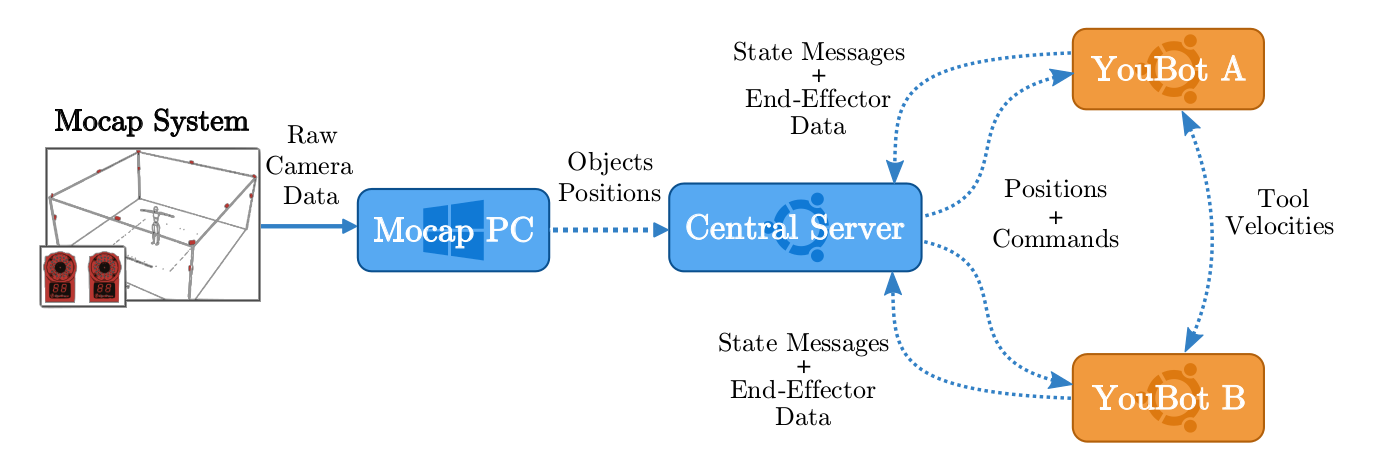
\includegraphics[scale=0.32]{systemArch}
			\captionof{figure}{\small \textit{Overall setup scheme, where the arrows indicate the UDP data flow, wired (solid) and wireless(dotted)}}
			\label{fig:systemArch}
		\end{figure*}
		
		\captionsetup[subfigure]{labelformat=empty}
		
		\begin{figure*}[b!]
			
			\begin{subfigure}{.5\linewidth}
				\hspace{-30px}
				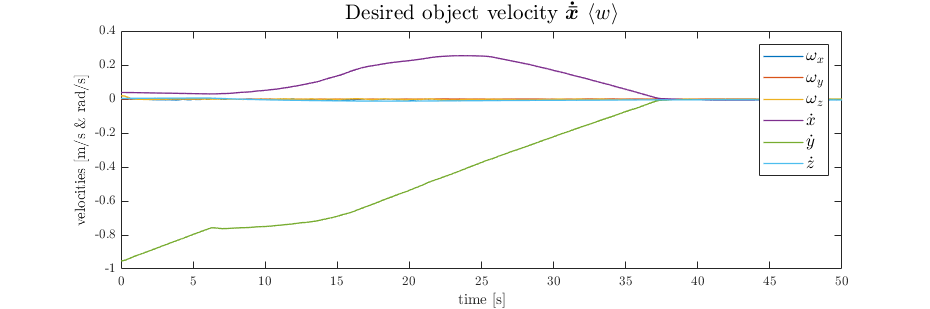
\includegraphics[width=280px,height=100px]{desiredvel}
				\caption{\hspace{-15px}(a)}
				\label{fig::a}
			\end{subfigure}
			\hfill
			\begin{subfigure}{.5\linewidth}
				\hspace{-10px}
				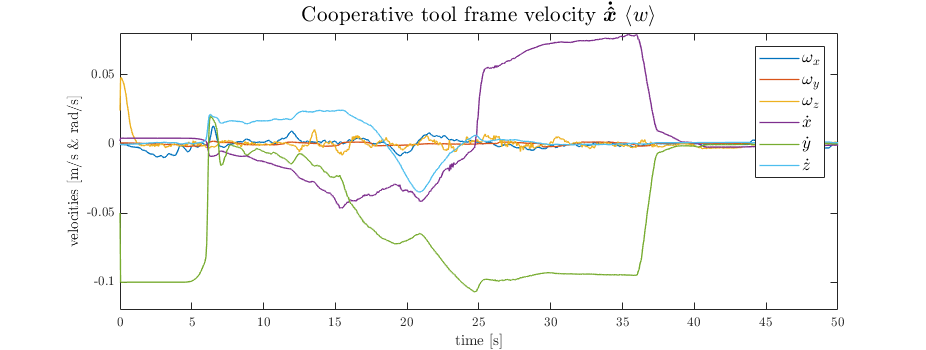
\includegraphics[width=280px,height=100px]{coopab}
				\caption{\hspace{25px}(b)}
				\label{fig::b}
			\end{subfigure}
	
			\vspace{10px}
			\begin{subfigure}{.5\linewidth}
				\hspace{-30px}
				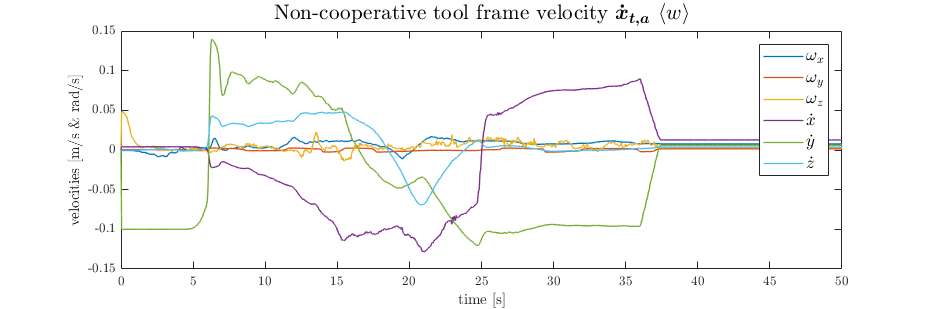
\includegraphics[width=280px,height=100px]{noncoopa}
				\caption{\hspace{-15px}(c)}
				\label{fig::c}
			\end{subfigure}
			\hfill
			\begin{subfigure}{.5\linewidth}
				\hspace{-10px}
				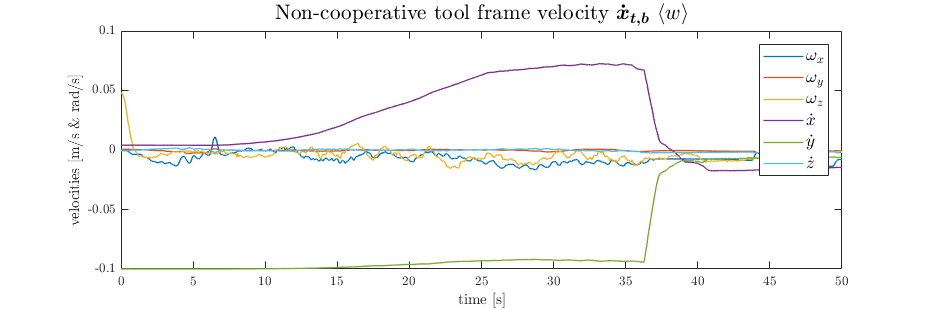
\includegraphics[width=280px,height=100px]{noncoopb}
				\caption{\hspace{25px}(d)}
				\label{fig::d}
			\end{subfigure}
			
		\end{figure*}
			 
		\section{Experimental Results} \label{sec:res}
		In this section we present the system architecture, as we can see in Fig.\ \ref{fig:systemArch} and the results obtained with the proposed kinematic control strategy.
		
		\subsection{System Setup}
		\hspace{7px}The odometry of the wheels,  in general, is not precise and, for the collaboration, the agents have to know the position of each other and their position respect to the world frame; we need an external view to understand where the robots are located. So the environment where the robots work is fully observed by 8 OptiTrack Flex3 cameras which detect the 6 markers putted on each robot. The MoCap PC with Motive software constructs the two rigid bodies of the robots from the 6 markers and sends their position to the central server via UDP.\\The central server is the master which sends the relevant data to the two youBots and it serves the purpose of being a unified console for controlling the two agents. 
		
		\setcounter{figure}{6}
		\begin{figure*}[t!]
			
			\begin{subfigure}{.5\linewidth}
				\hspace{-30px}
				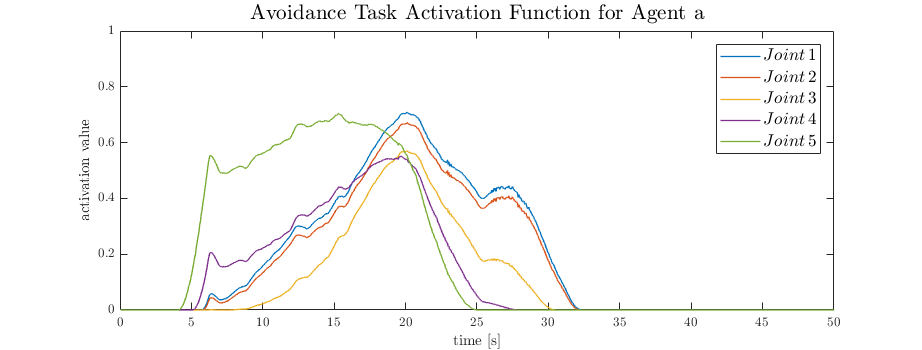
\includegraphics[width=280px,height=100px]{ActivationFunction}
				\caption{\hspace{-15px}(e)}
				\label{fig::e}
			\end{subfigure}
			\hfill
			\begin{subfigure}{.5\linewidth}
				\hspace{-10px}
				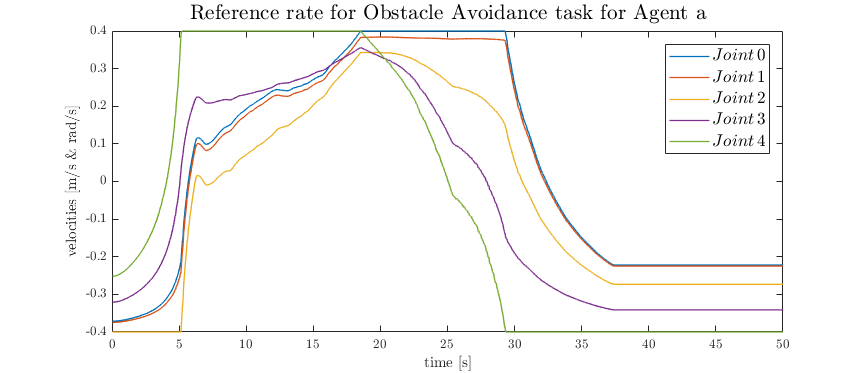
\includegraphics[width=280px,height=100px]{RefObstaclea}
				\caption{\hspace{25px}(f)}
				\label{fig::f}
			\end{subfigure}
			
			\caption{\small \textit{Results: }(a)\textit{ the desired object velocity, }(b)\textit{ cooperative tool-frame velocities (tuned toward agent} a \textit{, }(c)\textit{ non-cooperative tool-frame velocities for agent} a \textit{, }(d)\textit{ non-cooperative tool-frame velocities for agent} b \textit{, }(e)\textit{ avoidance task activation function for agent} a \textit{, }(f)\textit{ reference rate for avoidance task for agent} a.}
			
			\label{fig::results}
		\end{figure*}
		
		\subsection{Obtained Results}
		At the beginning of the graphs the two youBots are in a configuration similar to the one represented in Fig.\ \ref{fig:youBots}. Please note that, due to the MoCap system frame, the final position has negative component on $y$ axes; so the velocity needed on $y$ must be negative.\\
		In the Fig.\ \ref{fig::a} we can see the desired object velocity $\dot{\bar{\boldsymbol{x}}}$ calculated to make the tool reaching a desired position without considering the obstacle.\\
		As the robots go on, we can see in Fig.\ \ref{fig::c} (t = 6$s$) that the TPIK procedure of agent \textit{a} generates a non-cooperative tool frame velocity $\dot{\boldsymbol{x}}_{t,a}$ to make it go around the obstacle. Instead, the non-cooperative tool frame velocity $\dot{\boldsymbol{x}}_{t,b}$ in Fig.\ \ref{fig::d} is similar to the desired one because the agent \textit{b} does not meet any difficulties in its action.
		So, due to the fact that the non-cooperative velocity of agent \textit{a} is very different with respect to the desired one, the cooperative tool frame velocity $\dot{\hat{\boldsymbol{x}}}$ in Fig.\ \ref{fig::b} is tuned toward the agent \textit{a} which is in more trouble tracking the desired velocity. The presence of the obstacle is shown by the fact that the avoidance task activation function is greater than zero, as depicted in Fig.\ \ref{fig::results}\color{blue}e\color{black}.\\ 
		The Fig.\ \ref{fig::results}\color{blue}f \color{black} shows the agent \textit{a} reference rate generated by the obstacle avoidance task.
		
		\section{Conclusions} \label{sec:conc}
		We see that the TPIK methods proposed in \cite{tpik} and in \cite{coopcasa} are very efficient to implement the various tasks such as the obstacle avoidance task. The modular architecture developed in \cite{wander} makes this work simple and proficient as seen in the results \ref{sec:res}. \\
		\hspace*{7px}A further work could consist in the obstacle recognition by the MoCap cameras or by robot sensors which must be added to the agents. \\
		\hspace*{7px}This work is part of a cooperation with another research group which has developed an alignment task. Being both part of a bigger project, the two assignments can be merged to continue the project of the robot cooperative transportation in difficult environments. 

		
		\renewcommand\refname{\large{Reference}}
		\begin{thebibliography} {9}
			\vspace{-7px}
			\small
			
			\bibitem{subvec}
			E. Simetti, G. Casalino. 
			\textit{Manipulation and transportation with cooperative underwater vehicle manipulator systems}.
			IEEE Journal of Oceanic Engineering, 2016.	
			
			\bibitem{tpik}
			E. Simetti, G. Casalino. 
			\textit{A novel practical technique to integrate in equality control objectives and task transitions in priority based control}.
			Journal of Intelligent \& Robotic Systems, 2016.
			
			\bibitem{coopcasa}
			E. Simetti, G. Casalino, F.Wanderlingh. 
			\textit{A novel practical technique to integrate in equality control objectives and task transitions in priority based A Task Priority Approach to Cooperative Mobile Manipulation: Theory and Experiments}.
			Submitted for publication, 2018.	
			
			\bibitem{wander}
			F.Wanderlingh. 
			\textit{Cooperative Robotic Manipulation for the Smart Factory}.
			Università degli Studi di Genova, 2018.
			
			\bibitem{kuka}
			KUKA. 
			\textit{KUKA youBot User Manual}.
			Locomotec, 2012.
			
		\end{thebibliography}


	\end{multicols}	


\end{document}